\documentclass[../report.tex]{subfiles}
\begin{document}
    \begin{frame}
        \frametitle{1a: Average face}
        \begin{figure}[!htb]
            \centering
            \frame{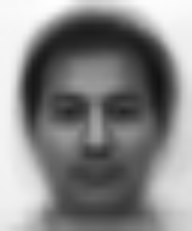
\includegraphics[keepaspectratio,height=0.65\textheight,width=0.45\textwidth]{ps6-1-a-1}}
            \caption{ps6-1-a-1} 
        \end{figure}
    \end{frame}

    \begin{frame}
        \frametitle{1b: Eigenvectors}
        \begin{figure}[!htb]
            \centering
            \frame{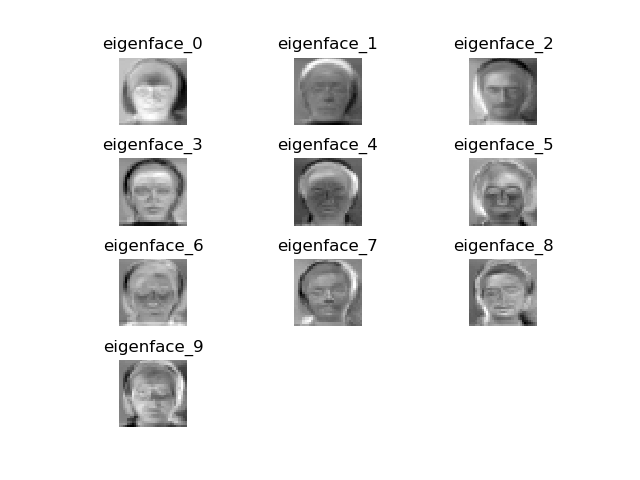
\includegraphics[keepaspectratio,height=0.65\textheight,width=0.45\textwidth]{ps6-1-b-1}}
            \caption{ps6-1-b-1} 
        \end{figure}
    \end{frame}

    \begin{frame}[t]
        \frametitle{1c: Analysis}
        \begin{normalsize}
            \begin{itemize}
                \setlength\itemsep{1em}\fontsize{6pt}{6pt}

                \item[]{\textbf{\selectfont\textcolor{blue}{ Analyze the accuracy results over multiple iterations. Do these “predictions” perform better than randomly selecting a label between 1 and 15? Are there any changes in accuracy if you try low values of k? How about high values? Does this algorithm improve changing the split percentage p? }}}
                
                \item[]\textbf{The predictions perform better than randomly selecting a lable between 1 and 15\\
For low values of K, accuracy is greatly reduced.  \\
The algorithm does not seem sensitive to changing the split percentage. \\
Although it can be hard to tell due to standard deviation of the results. \\
}
            \end{itemize}
        \end{normalsize}
    \end{frame}
    
\end{document}